\documentclass[oneside,a4paper,12pt]{memoir}
\usepackage{amssymb,amsmath}
\usepackage{chngcntr}
\usepackage{color}
\usepackage[latin1]{inputenc}
\usepackage[ruled,vlined,linesnumbered]{algorithm2e}
\usepackage{graphicx}
%\usepackage{caption}
\usepackage{subcaption}
\usepackage{url,hyperref}
\usepackage{booktabs}
\usepackage{float}
\usepackage{colortbl}
\usepackage{comment}
\usepackage{ulem}
\usepackage{todonotes}

\begin{document}
\title{SAIM - Manual}
\author{Klaus Lyko}                                                  
\maketitle

\newpage
\tableofcontents*
\chapter{Introduction}
Links between instance are of central importance for the Semantic Web and for a large number of tasks, such as data integration, federated querying and knowledge retrieval. Finding those links is the subject of Link Discovery (LD).
Two main problems arise when trying to discover links between data sets.

First, naive solutions have to compare all instances of a source knowledge base with all instances of the target knowledge base, thus having a quadratic time complexity. Second, one have to guarantee the quality of those links. 
To address the first problem time efficient algorithms and frameworks such as SILK\footnote{\url{https://www.assembla.com/spaces/silk/}} and LIMES\cite{NGAU11} have been developed to reduce the number of comparisons. For the second problem both supervised (e.g. \cite{NGLY12, NGO+13}) and unsupervised ({e.g. \cite{NIK+12}}) machine learning approaches have been developed.

SAIM \footnote{SAIM stands for (\uline{S}emi-)\uline{A}utomatic \uline{I}nstance \uline{M}atcher.}  encompasses solutions for both problems within one interface. It is based upon algorithms implemented in the LIMES\footnote{\url{http://limes.sf.net/}} framework which have been shown to outperform state-of-the-art in previous work w.r.t. time-complexity \cite{NGON12c}. SAIM offers an intuitive GUI for experts to manually create Link Specifications while implementing the supervised and unsupervised machine learning algorithms EAGLE \cite{NGLY12}	and COALA \cite{NGO+13} respectively, which have been shown to lead to highly accurate link specifications.

This manual will cover the complete workflow of SAIM. Starting in chapter \ref{kbdefinition} from scratch it will cover the process of defining the endpoints(\ref{endpoint}), class restrictions(\ref{classes}) and properties(\ref{properties}) of the knowledge bases to link. Chapter \ref{manual} describes how experts can build link specifications manually. Chapter \ref{selfconfig} and \ref{learning} discusses the unsupervised and supervised learning algorithms respectively. Finally, chapter \ref{features} covers additional features of SAIM such as saving and loading link specifications, uploading RDF dumps.

%%%%%%%%%%%%%%%%%                                  ENDPOINTS 													%%%%%%%%%%%%%%%%%%%%%%%%%
\chapter{Source and Target Endpoint definition}
\label{kbdefinition}
	Figure \ref{fig:MainWindow} shows SAIM upon startup.
	\begin{figure}
		\centering
		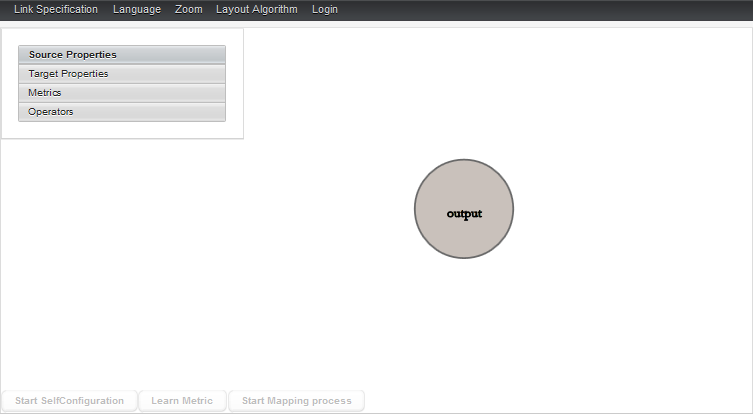
\includegraphics[width=0.8\textwidth]{images/main.png}
		\caption{The main window of SAIM is divided into three parts: A \emph{menu bar} at the top, an \emph{accordion} panel to the left and the \emph{metric panel} at the center.}
		\label{fig:MainWindow}
	\end{figure}
	As all no link specification is defined yet the 3 buttons at the bottom are deactivated and the accordion panel is empty. To start a Link Specification we go to the menu \texttt{Link Specification}. Figure \ref{fig:menu_start} shows the available menu entries:	
	\begin{enumerate}
		\item \texttt{Start new configuration} Start a new Link Specification from scratch.
		\item \texttt{Import Link Specification} To Import Link Specifications. It is covered in section \ref{ImportExport}.
		\item \texttt{Export Link Specification} Let you save Link Specifications on you local machine. It is covered in section \ref{ImportExport}.
		\item \texttt{Info} Will open a window with basic information about us.
	\end{enumerate}
	\begin{figure}
		\centering
		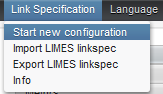
\includegraphics{images/menu_start.png}
		\caption{The \texttt{Link specification} menu.}
		\label{fig:menu_start}
	\end{figure}
	
	\section{Endpoints}
	\label{endpoint}
	To start a link specification we have to specify the RDF data sources dubbed \textit{Source} and \textit{Target Endpoint}. To do so go in the menu bar to \texttt{Link Specification} $>>$ \texttt{Start new configuration} as depicted in figure \ref{fig:menu_start}. This will open a Window as shown in figure \ref{fig:endpoint}. \\
	There are fields to be set:
	\begin{enumerate}
		\item \texttt{Endpoint URL} The URL of the public accessible SPARQL endpoint.
		\item \texttt{ID/Namespace} identifies the endpoint. Should be a string differentiating the endpoint as this entry is used be certain class matchers later.
		\item \texttt{Graph} (optinal) URI of a specify RDF graph.
		\item \texttt{Page Size} (optional) For pagination of SPARQL queries.
	\end{enumerate}
	It is possible to use predefined Presets from a list, such as DBPedia as depicted in the top layer of figure \ref{fig:endpoint}. SAIM also supports RDF local dumps on the Server. We have loaded the OAEI2010\footnote{Ontology Alignment Evaluation Initiative: \url{http://oaei.ontologymatching.org/2010/}} Benchmark datasets Person1, Persons2 and Restaurants. These datasets are accessible via the \texttt{Preset} list. SAIM supports the upload of RDF dumps in diffferent formats. Please refer to section \ref{upload} for details.\\
	\begin{figure}[!h]
		\centering
		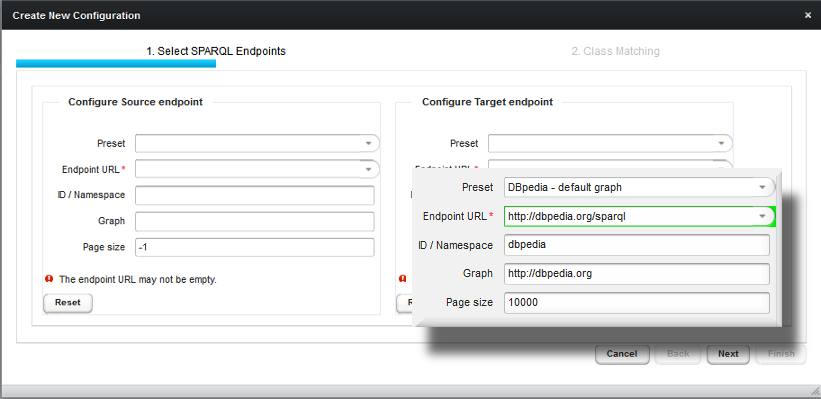
\includegraphics[width=0.95\textwidth]{images/endpoint.png}
		\caption{The Panel to specify the SPARQL endpoints. The front layer shows an example configuration to use DBPedia as an endpoint.}
		\label{fig:endpoint}
	\end{figure}
If a public accessible SPARQL endpoint is used instead, SAIM tests its availability by issueing a simple SPARQL query. If the test for reachability is successful SAIM indicates it by a green margin arround the \texttt{Endpoint URL} field as indicated in the top layer of figure \ref{fig:endpoint}.
	\section{Class restriction}
	\label{classes}
	\section{Property Matching}
	\label{properties}
%%%%%%%%%%%%%%%%                              MANUAL LINK SPECS 											%%%%%%%%%%%%%%%%%%%%%%%%%
\chapter{Manual metric definition and execution}
\label{manual}

%%%%%%%%%%%%%%%%%                             SELFCONFIGURATION 											%%%%%%%%%%%%%%%%%%%%%%%%%
\chapter{Selfconfiguration}
\label{selfconfig}

%%%%%%%%%%%%%%%%%                                  LEARNING 													%%%%%%%%%%%%%%%%%%%%%%%%%
\chapter{Improving results through learning}
\label{learning}

%%%%%%%%%%%%%%%%%                                  FEATURES 													%%%%%%%%%%%%%%%%%%%%%%%%%
\chapter{Additional features}
\label{features}
\section{Import and save Link Specifications}
\label{ImportExport}

\section{Uploading RDF dumps}
\label{upload}

\bibliographystyle{plain}
\bibliography{saim}

\newpage
\appendix
\chapter{}
\section{The menu bar}
\label{menuBar}

\end{document}